\newcommand{\files}[1]{
    \hfill
    \mbox{
        $\hookrightarrow$
        \texttt{#1}
    }
}

\section{Lautsprecher}
\label{sec:1}
\blindtext

\def\arraystretch{1.3}
\begin{table}[h]
    \centering
    \caption{Eine Tabelle}
    \label{tab:mics}
    \begin{tabular}{l l l l l}
        Hersteller & Typ & Akustische Arbeitsweise & Richtcharakteristik & Einfallsrichtung \\
        \hline
        Shure & \texttt{SM58} & Druckgradienten-/Schnelleempfänger & Niere & 0°, 90°, 180° \\
    \end{tabular}
\end{table}


\subsection{Abstrahlcharakteristik}
\label{subsec:a}
Abbildung \ref{fig:balloon} zeigt die Abstrahlcharakteristik eines Cellos bei verschiedenen Frequenzen in Oktavabstand.
Für eine anschauliche Darstellung wurden die Werte so normiert, dass der niedrigste Wert auf 20 dB liegt.
Mit steigender Frequenz ist zu erkennen, dass die Schalldruckpegelwerte im allgemeinem abnehmen.
Darüber hinaus deformiert sich die zunächst sphärische Form des Ballons zu den hohen Frequenzen hin mit hervortretenden bzw. hineinragenden Beulen.
Daher scheint die Ausbreitung der Schalldruckpegel bei niedrigen Frequenzen nahezu kugelförmig zu sein.
Bei hohen Frequenzen wird zunehmend die für ein Cello charakteristische Abstrahlrichtung erkennbar - leicht schräg nach oben (orthogonal zu den F-Löchern des Resonanzkörpers) und horizontal in die breite gehend.
Schallabsorbierende Hindernisse vom Cellisten und dem Cello selbst haben auch Einfluss auf die Ausbreitung des Schalldruckpegel.
So ist über alle Frequenzen hinweg ein Abfall des Schalldruckpegel nach hinten, im Schatten des Cellisten, erkennbar.
Bei hohen Frequenzen mit kurzer Wellenlänge lässt sich eine kleine Lücke, vermutlich durch die spielenden Hand und den Bogen verursacht, vermuten.


\begin{figure}[bth]
    \centering
    \begin{subfigure}{.5\textwidth}
        \centering
        \caption{125 Hz}
        \includegraphics[width=0.80\linewidth]{Figures/125Hz.eps}
    \end{subfigure}%
    \begin{subfigure}{.5\textwidth}
        \centering
        \caption{250 Hz}
        \includegraphics[width=0.80\linewidth]{Figures/250Hz.eps}
    \end{subfigure}

    \vspace{0.5cm}
    \begin{subfigure}{.5\textwidth}
        \centering
        \caption{500 Hz}
        \includegraphics[width=0.80\linewidth]{Figures/500Hz.eps}
    \end{subfigure}%
    \begin{subfigure}{.5\textwidth}
        \centering
        \caption{1000 Hz}
        \includegraphics[width=0.80\linewidth]{Figures/1000Hz.eps}
    \end{subfigure}

    \vspace{0.5cm}
    \begin{subfigure}{.5\textwidth}
        \centering
        \caption{2000 Hz}
        \includegraphics[width=0.80\linewidth]{Figures/2000Hz.eps}
    \end{subfigure}%
    \begin{subfigure}{.5\textwidth}
        \centering
        \caption{4000 Hz}
        \includegraphics[width=0.80\linewidth]{Figures/4000Hz.eps}
    \end{subfigure}

    \vspace{0.5cm}
    \begin{subfigure}{.5\textwidth}
        \centering
        \caption{8000 Hz}
        \includegraphics[width=0.80\linewidth]{Figures/8000Hz.eps}
    \end{subfigure}

    \caption{Abstrahlcharakteristik eines Cellos bei verschiedenen Frequenzen in Oktavabstand}
    \label{fig:balloon}
\end{figure}


\subsection{Frequenzgang}
\label{subsec:b}
\blindtext


\subsection{SPH-450TC Treiber}
\label{subsec:c}

Die zur Berechnung des Frequenzgangs benötigten Thiele-Small-Parameter wurden dem Datenblatt \cite{SPH-450TC} des SPH-450TC Treibers entnommen.

\begin{itemize}
  \item Resonanzfrequenz $f_s$ = 20 Hz
  \item Gesamtgüte $Q_{ts}$ = 0,25
  \item Äquivalentvolumen $V_{as}$ = 480 l
\end{itemize}

Mit Hilfe der folgenden Formel (2) aus der Aufgabenstellung wurde die Resonanzkreisfrequenz $\omega_c$ berechnet.
Wie gefordert wurde für $Q_{ts}$ der Wert $\frac{1}{\sqrt{2}}$ verwendet.

\[
\omega_c = \frac{Q_{tc}}{Q_{ts}} \cdot \omega_s 
\]

Die Lösung der Gleichung ergab ein $\omega_c$ von $355.4 \frac{1}{s}$ (56.5 Hz). 
Mit diesem Ergebnis und den Werten aus dem Datenblatt lässt sich nun das benötigte Gehäusevolumen errechnen.
Dafür wurde die Formel (3) aus der Aufgabestellung verwendet.

\[
V_b = \frac{V_{as}} {\left( \frac{\omega_c}{\omega_s} \right) ^{2} - 1}
\]

Das berechnete Gehäusevolumen  $V_b$ beträgt 68,57 Liter.
Der resultierende Amplitudenfrequenzgang ist in Abbildung \ref{fig:Normaler_Frequenzgang} zu sehen.
Die Resonanzfrequenz $f_c$ wurde in der Abbildung mit einem roten Kreis markiert. 
Die -3 dB Cutoff-Frequenz wurde mit einem roten Sternchen markiert.
In diesem Fall liegen beide Werte aufeinander.

\begin{figure}[H]
    \centering
    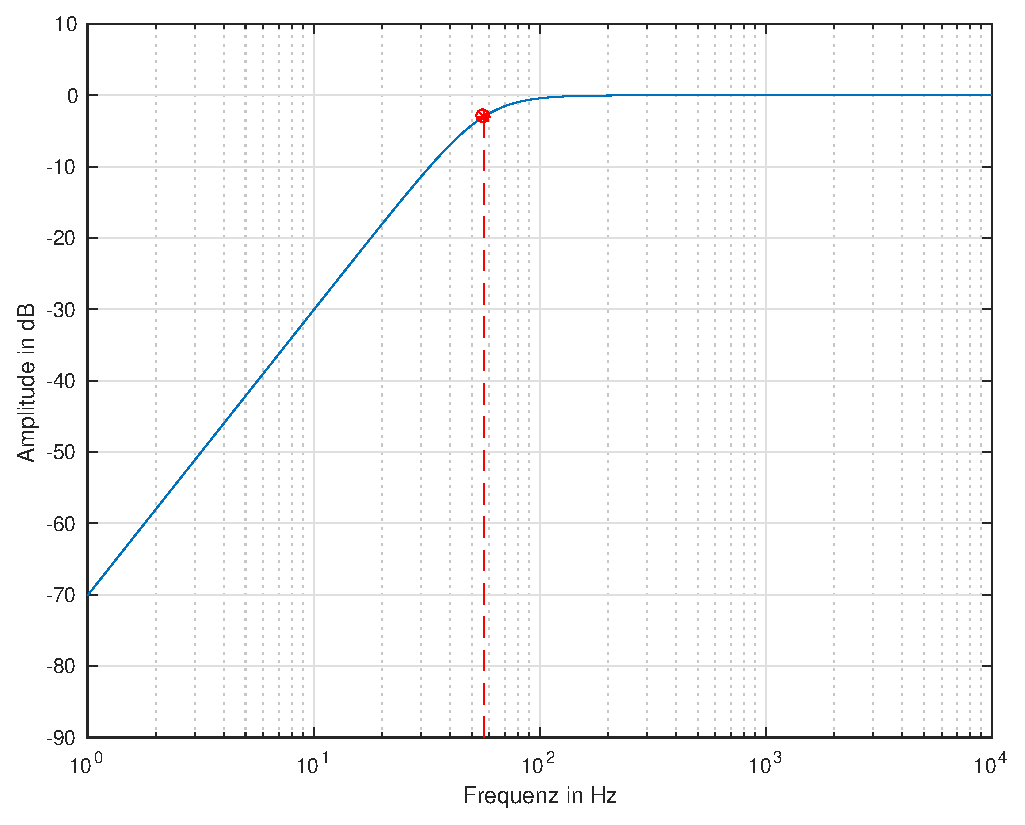
\includegraphics[width=0.7\textwidth]{Figures/Normaler_Frequenzgang.eps}
    \caption{Normaler Amplitudenfrequenzgang}
    \label{fig:Normaler_Frequenzgang}
\end{figure}%

Anschließend sollten die Gehäusevolumen $V_{b,3}$ und $V_{b,1}$ ermittelt werden, welche zu einer maximalen Überhöhung des Betragfrequenzgangs von 3 dB bzw. 1 dB respektive führt.
Dies wurde in einem iterativen Prozess umgesetzt.
Die resultierenden Frequenzgänge sind in Abbildung \ref{fig:Ueberhoehung} zu sehen.
Wie in der vorhergehenden Abbildung ist die Resonanzfrequenz $f_c$ mit einem roten Kreis und die -3 dB Cutoff-Frequenz mit einem roten Sternchen markiert.
Der berechnete Wert von $V_{b,3}$ liegt bei 18 Litern mit einer Güte $Q_{ts}$ von 1.32.
Für $V_{b,1}$ wurde ein Wert von 35 Litern und eine Güte von 0.96 errechnet.

\begin{figure}[H]
    \centering
    
    \begin{subfigure}{.49\textwidth}
        \centering
        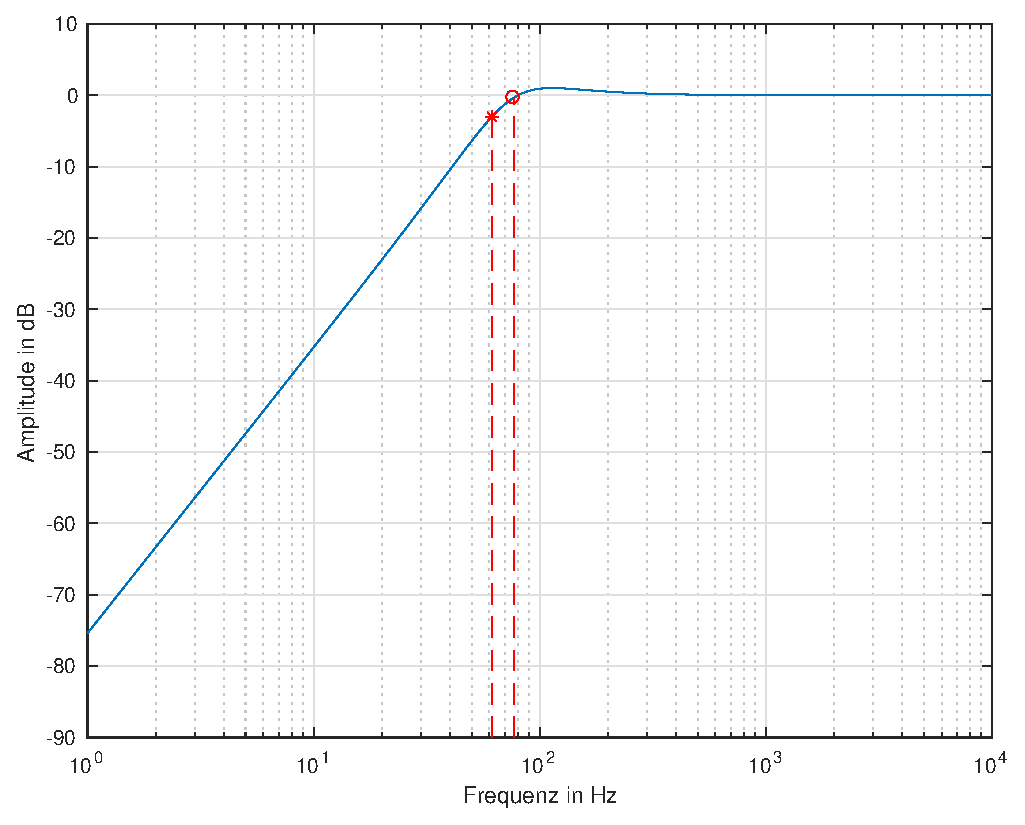
\includegraphics[width=0.85\linewidth]{Figures/Frequenzgang_1dB.eps}
        \caption{1dB Überhöhung}
        \label{Frequenzgang_1dB}
    \end{subfigure}
    \begin{subfigure}{.49\textwidth}
        \centering
        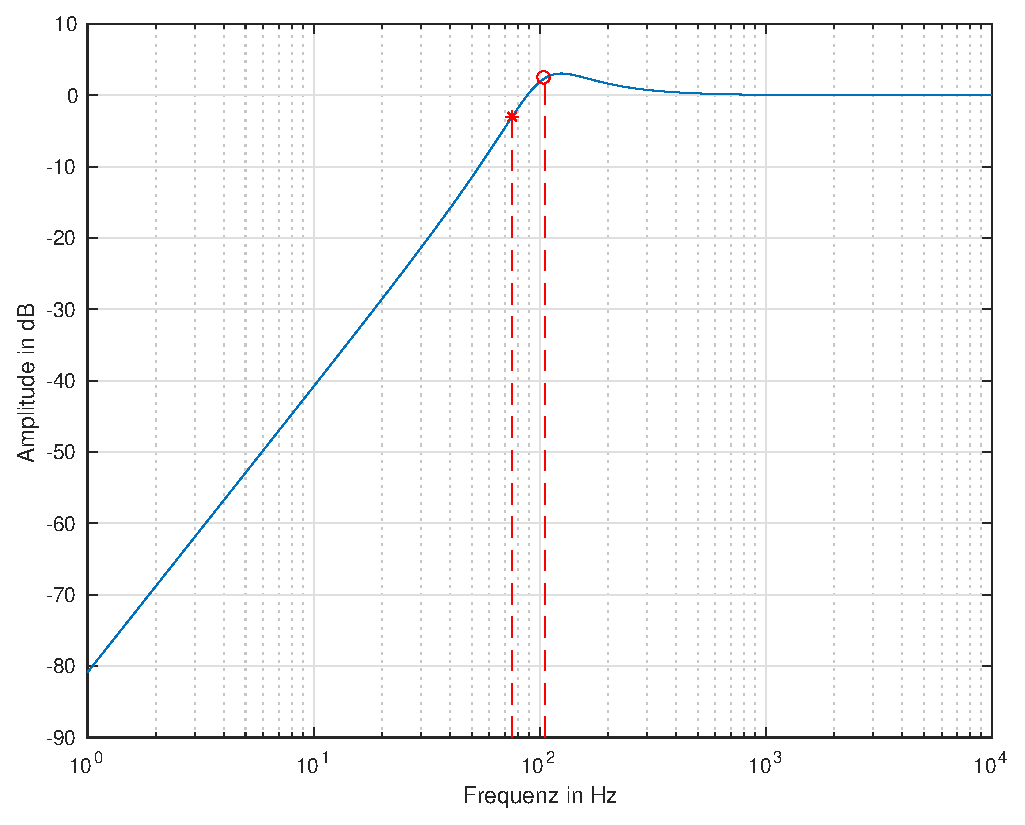
\includegraphics[width=0.85\linewidth]{Figures/Frequenzgang_3dB.eps}
        \caption{3dB Überhöhung}
        \label{Frequenzgang_3dB}
    \end{subfigure}
    
    \caption{Frequenzgänge mit verschiedenen Überhöhungen}
    \label{fig:Ueberhoehung}
\end{figure}